\documentclass{article}
\usepackage[utf8]{inputenc}
\usepackage{algpseudocode}
\usepackage{algorithm}
\usepackage{tikz}
\usepackage{amsmath}
\usetikzlibrary{automata}

\title{Algorithmique Avancée TD01}
\author{Hugo Demaret}
\date{September 2021}
\begin{document}
\maketitle
\section*{Partie A -}
\section*{Partie B -}
Voir sur :\\
	https://github.com/HugoDemaret/linked\_list\\
	https://github.com/HugoDemaret/doublelinked\_list\\
	https://github.com/HugoDemaret/binary\_tree\\

\section*{Partie C -}
\subsection*{Exercice 1 -}
	\textbf{Déterminons quelle est la complexité asymptotique de cet algorithme.}\\\\
\subsection*{Exercice 2 -}
	\textit{Soit T un graphe avec n sommets. Démontrer que les propriétés suivantes sont équivalentes.}\\\\
	\textbf{(1) T est un arbre}\\
	\textit{La définition d'un arbre est : Graphe acyclique et connexe.}\\\\
	\textbf{(2) T est un graphe connexe et acyclique}\\
	\textit{C'est en fait l'une des définitions d'un arbre.}\\\\
	\textbf{(3) T est un graphe connexe avec n-1 arrête}\\
	\textit{Un graphe cyclique à n sommets possède au minimum n arrêtes. Donc un graphe connexe à n-1 		arrêtes est acyclique. C'est un arbre.}\\\\
	\textbf{(4) T est un graphe acyclique avec n-1 arrête}\\
	\textit{T est un graphe simple. Un graphe acyclique est un graphe simple (la boucle serait un cycle). Le graphe possède n-1 arrêtes, donc chaque sommet possède au moins une arrête (parfois en commun avec un autre sommet). Donc le graphe est connexe. C'est donc un arbre.}\\\\
\textit{Les propriétés précédentes décrivant toutes un arbre, elles sont équivalentes.}\\\\
\subsection*{Exercice 3 -}
\textit{Considérons 3 définitions d'un arbre : }\\\\\\

\textit{Définition 1.}\\
\textsf{Un arbre T est un graphe :}\\
\textsf{• Qui est simple (sans boucle)}\\
\textsf{• Tel que : }\\
\begin{equation}
\forall (u,v) \in T, u \neq v, \exists! \eta[u,v]
\end{equation}\\
\textsf{Cette définition repose sur les deux propositions suivantes :}\\
\textit{Proposition 1 : S'il y a un chemin de v à w dans le graphe G, alors il y a aussi un chemin simple de v à w.}\\
\textit{Proposition 2 : S'il y a un cycle dans G, alors il y a un cycle simple dans G.}\\\\\\

\textit{Définition 2.}\\
\textsf{Un graphe non-orienté connexe et acyclique est appelé un arbre.}\\\\\\

\textit{Définition 3.}\\
\textsf{Un arbre est un graphe connexe minimal. C'est-à-dire que toute suppression d'arrêtes le rend non connexe.}\\\\\\

\section*{Partie D -}
\subsection*{Exercice 1.1 -}
\textit{Soit G le graphe suivant :}\\\\\\
\begin{center}
	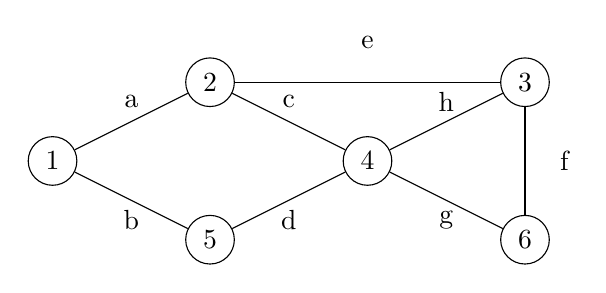
\begin{tikzpicture}
	\node[circle,draw=black] (v1) at (0,0) {1};
	\node[circle,draw=black] (v2) at (2,1) {2};
	\node[circle,draw=black] (v5) at (2,-1) {5};
	\node[circle,draw=black] (v4) at (4,0) {4};
	\node[circle,draw=black] (v3) at (6,1) {3};
	\node[circle,draw=black] (v6) at (6,-1) {6};
	\node[] (a) at (1,0.75) {a};
	\node[] (b) at (1,-0.75) {b};
	\node[] (e) at (4,1.5) {e};
	\node[] (c) at (3,0.75) {c};
	\node[] (d) at (3,-0.75) {d};
	\node[] (h) at (5,0.75) {h};
	\node[] (g) at (5,-0.75) {g};
	\node[] (f) at (6.5,0) {f};
	\draw[](v1)--(v2);
	\draw[](v2)--(v3);
	\draw[](v3)--(v4);
	\draw[](v2)--(v4);
	\draw[](v4)--(v5);
	\draw[](v5)--(v1);
	\draw[](v3)--(v6);
	\draw[](v6)--(v4);
	\end{tikzpicture}
\end{center}
	\textit{Matrice d'adjacence de G :}\\
	\begin{center}
	$
	A =
	\left[\begin{matrix}
		0&1&0&0&1&0\\
		1&0&1&1&0&0\\
		0&1&0&1&0&1\\
		0&1&1&0&1&1\\
		1&0&0&1&0&0\\
		0&0&1&1&0&0
	\end{matrix}\right]
	$
	\end{center}
	\textit{Codage en liste d'arrêtes et sommets :}
	\begin{table}[h]
		\begin{center}
		\begin{tabular}{|c | c | c | p{5cm}}
		\hline
		Sommet & arrêtes & sommets\\
		\hline \hline
		1&a,b&2,5\\
		2&a,c,e&1,3,4\\
		3&e,f,h&2,4,6\\
		4&c,d,g,h&2,3,5,6\\
		5&b,d&1,4\\
		6&f,g&3,4\\
		\hline
		\end{tabular}
		\end{center}
	\end{table}
\subsection*{Exercice 1.2 -}
\textit{On considère G un graphe simple et non dirigé.}\\\\
\textbf{1 -}
\textit{Soit A la matrice d'adjacence de G. Que valent les sommes par lignes et par colonnes ?}\\\\
\textsf{Les sommes par lignes et par colonnes nous donnent le degré des sommets de G.}\\\\
\textbf{2 -}
\textit{Soit M la matrice d’incidence de G, c’est-à-dire une matrice de taille $\big|V(G)\big| \cdot \big|E(G)\big|$ telle que $m_{ue} = 1$ si l’arrête e est incidente au sommet u et $m_{ue} = 0$ sinon. Ecrire la matrice d’incidence du graphe de l’exercice précédent.}\\\\
\textit{Matrice d'incidence de G :}\\\\
\begin{center}
	$
	M =
	\left[\begin{matrix}
	1&1&0&0&0&0&0&0\\
	1&0&1&0&1&0&0&0\\
	0&0&0&0&1&1&0&1\\
	0&0&1&1&0&0&1&1\\
	0&1&0&1&0&0&0&0\\
	0&0&0&0&0&1&1&0
	\end{matrix}\right]
	$
\end{center}
\textbf{3 -}
\textit{Que valent les sommes des coefficients par lignes et par colonnes de M ?}\\\\
\textsf{La somme des coefficients par ligne de M nous donne le degré des sommets.}\\
\textsf{La somme des coefficients par colonne de M nous dit si le graphe est simple ou connexe.}\\\\
\textit{Somme par lignes :}\\\\
\begin{center}
$\sum_{}\big|M_{i}\big|$\\
\end{center}
\textit{Nous donne le degré du sommet i.}\\\\
\begin{center}
$max(\sum_{}\big|M_{i}\big|)$\\
\end{center}
\textit{Nous donne l'ordre du graphe.}\\\\\\
\textit{Somme par colonnes :}\\\\
\begin{center}
$\sum_{}\big|M_{j}\big| = \Bigg\{  \textit{si 1 : boucle (non-simple)}
\linebreak
\textit{- pas d'information sur la connexité}
\linebreak
\sum_{}\big|M_{j}\big| = \Bigg\{  
\textit{si 2 : arrête simple et connexe} \big. $
\end{center}
\textit{Nous dit si le sommet est simple, et s'il est connecté au reste du graphe.}\\\\
\textit{Min() somme par colonnes :}\\\\
\begin{center}
$\textit{min}(\sum_{}\big|M_{j}\big|) = \Bigg\{  \textit{si 1 : graphe non-simple} 
\linebreak
\textit{min}(\sum_{}\big|M_{j}\big|) = \Bigg\{  
\textit{si 2 : graphe simple et connexe} \big. $
\end{center}
\textit{Nous dit si le graphe est simple et connexe, ou s'il contient une boucle.}\\\\
\end{document}
